%3 背景・目的
\section{はじめに}
\subsection{背景}
遠隔地に自身が存在するかのような体験を可能にする, テレイグジスタンスという技術が存在する\cite{telexistence}.
この技術を利用し工場での作業やスポーツ観戦,旅行などを遠隔地から行う研究が行われてきた\cite{factorio}\cite{sprots}\cite{oculus}.

これらの研究の多くは図\ref{figure:Holopotation}のようなユーザの3Dモデル,または図\ref{figure:vrmodel}のようなロボッや完全没入型VRを利用することで自身の存在を遠隔地に投影させたり高い没入感で遠隔地で行動しているかのような体験を可能にしている\cite{vrmodel}\cite{ogasawara}.しかしこれらの手法においてユーザは移動しながら遠隔地での体験をすることはできない.ユーザの3Dモデルを利用する方法ではユーザ自身が深度情報を取得できるカメラに写っている必要があるためユーザの移動範囲に制限がある.
さらにロボットを用いた手法はユーザが完全没入型VRを利用する必要があり,ユーザは周囲の状況を把握することができないため移動しながらの利用はできない.

我々はこれらの問題を解決し実際に移動しながら遠隔地での体験を行うことでよりリアルな体験が可能になると考えた.
本研究では遠くにいる人と共に遠隔地の風景での行動を可能にする手法を提案する.そして提案した手法を基に遠くにいるユーザと共に遠隔旅行をするシステムの構築を行う.
本手法ではバーチャルヒューマンと呼ばれる仮想的な人間の3Dモデルをユーザのアバターとして使用することで自身の3Dモデル生成のための移動制限を無くす.更に出力に透過型MRヘッドマウントディスプレイを用いることで周囲の環境を認識し衝突などの危険性を抑制し,移動しならがリアルな体験を可能にする.

\begin{figure}[htbp]
\begin{center}
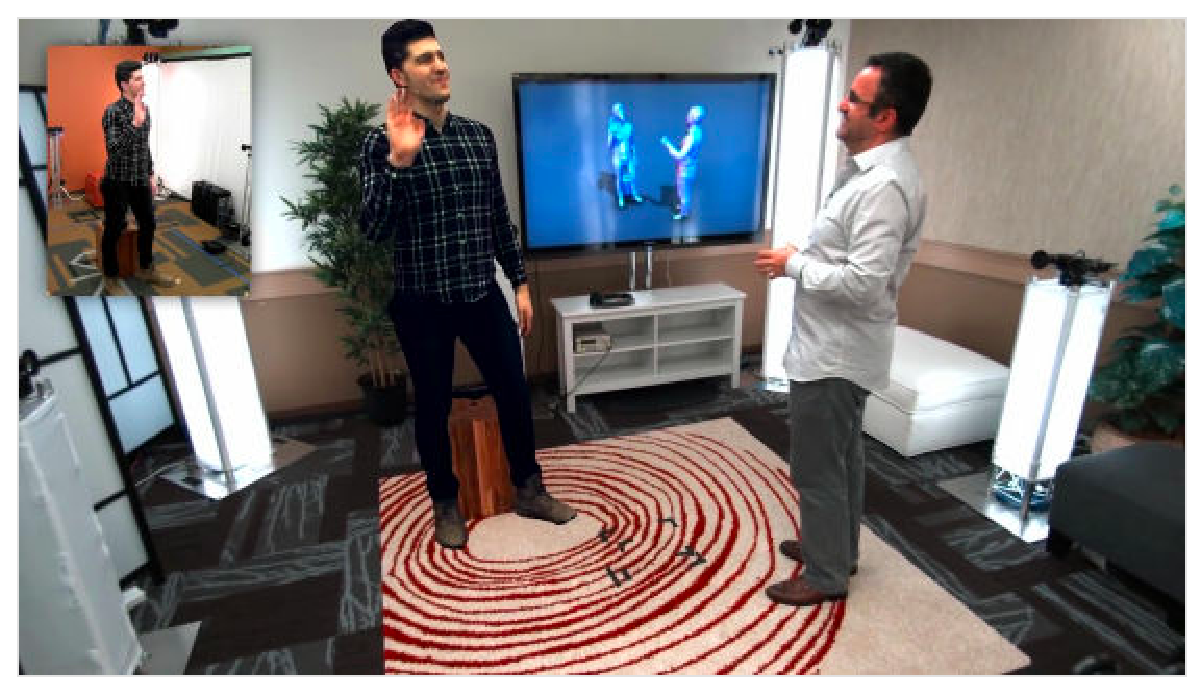
\includegraphics[width=16cm]{img/01_background/usermodel.eps} 
\end{center}
\caption{ユーザの3Dモデルを利用した手法}
\label{figure:Holopotation}
\end{figure} 

\begin{figure}[htbp]
\begin{center}
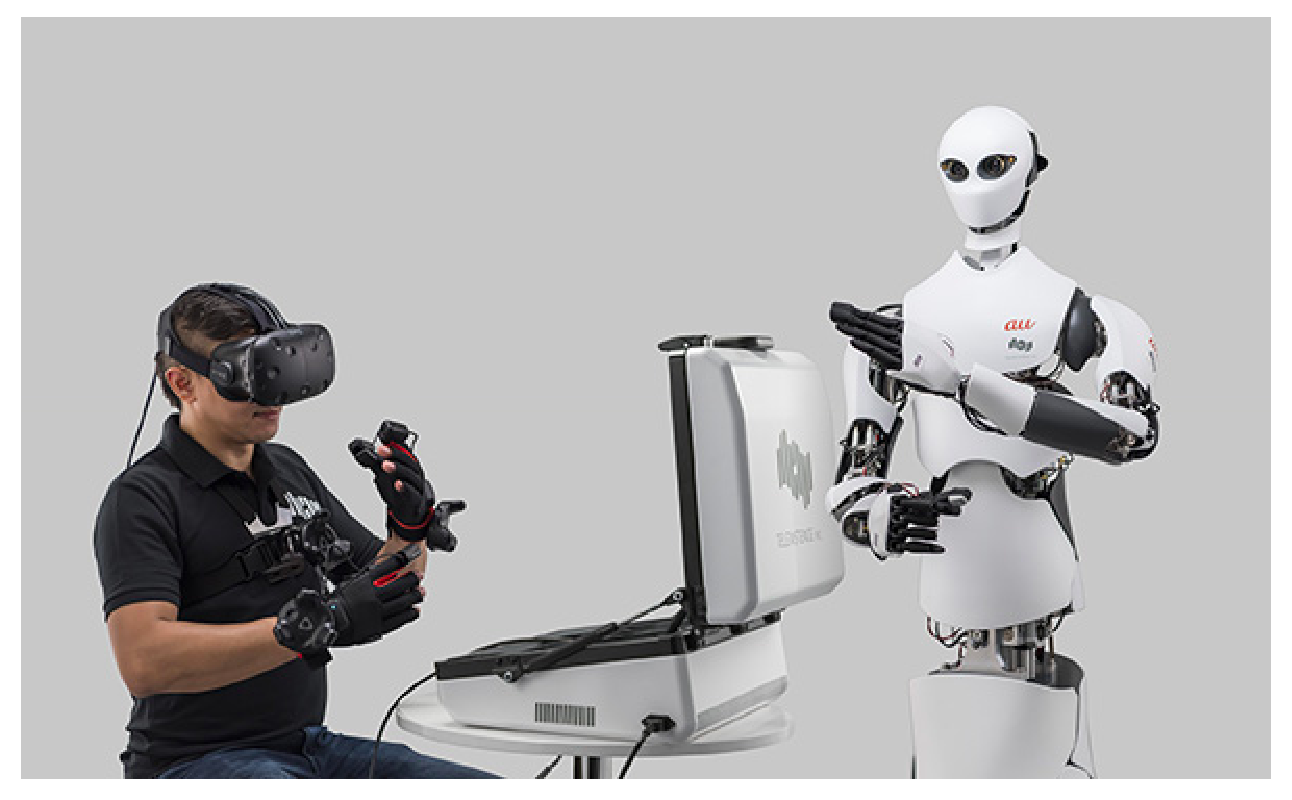
\includegraphics[width=16cm]{img/01_background/robovr.eps} 
\end{center}
\caption{ロボットや完全没入型VRを利用した手法}
\label{figure:vrmodel}
\end{figure} 

\clearpage

\subsection{目的}
本研究では移動を伴う環境において,テレイグジスタンスにより遠くにいる友人と,あたかも遠隔地で行動しているかのような体験をすることができる手法を提案し,提案手法を基に遠くにいるユーザと遠隔旅行をするシステムの開発を目的とする.

%睡眠不足は現代社会における深刻な問題である.

%睡眠不足によって記憶障害の原因となるたんぱく質が蓄積されることから, 睡眠不足はアルツハイマーの原因であると考えられている\cite{alzheimer}.
%さらに,睡眠時間が6時間以下の人は7時間の人に比べ死亡率が2.4倍になるという研究も存在する\cite{deadchance}.
%平成27年に厚生労働省が発表した調査では現代の日本人の40\%近くが睡眠時間6時間未満である.
%これは平成17年の調査結果より6\%増加しており, 日本人の睡眠時間は減少傾向にある\cite{undersix}.

%この問題の解決について, これまで様々なアプローチがとられてきた. だが, それらの多くは, 睡眠の「質」を向上させることを目的としている.
%代表的なものとして, レム睡眠, ノンレム睡眠のサイクルから最適なタイミングで起床を促す快眠支援アプリ「Runtastic Sleep Better」や, ユーザ固有の睡眠リズムから最適な音楽を流し睡眠の質を高める枕型デバイス「クローナ」などがある.

%我々は, この睡眠不足問題の改善のためには, 睡眠の「質」のみならず, 「量」をも重要視したアプローチをとることが重要であると考えた.

%なぜなら, ベネッセ教育総合研究所が行った調査「調査データクリップ!子どもと教育」において寝不足の理由の 50 \%以上が「なんとなく夜更かししてしまう」という結果が出たためである\cite{nebusoku}.
%「なんとなく夜更かししてしまう」のを改善するためには, ユーザに「寝なければいけない」という意識を持たせるよう働きかけること, 及び早めに就寝できるよう生活リズムを改善していくことが重要である.
%また, 「潜在的睡眠不足」と呼ばれる無自覚な睡眠不足に陥っている現代人が増加傾向にあることが, 国立精神・神経医療研究センターの調査により明らかとなっている\cite{psd}.
%潜在的睡眠不足に陥ると, 睡眠不足を自覚できないまま短時間の睡眠を繰り返し, 心身に負担を生じさせ続けてしまう. これの解消には, 睡眠の質を高めるアプローチよりも, 単純に長時間の睡眠を確保することが重要である.

%十分な睡眠時間を確保させるにはどうしたらよいか, という問題に対し, 我々は人々に時間を錯覚させることにより, 就寝時間を自然に早めさせることが可能なのではないか, という着想を得た.
%そこで我々は, 時間の錯覚効果が就寝時刻を早めるのに有効かどうか独自で調査を行った.

%調査協力者には, ゼミ活動での進捗報告会において時計を隠した状態で30分間過ごした後, アンケートで経過時間を回答してもらった. 男女 23 人を対象に調査を行った結果, 調査対象者の時間感覚に大きなばらつきが生じた.
%また, 日を改め, 時計を隠した状態で現在時刻を問い, そう思った理由を回答してもらったところ, 「ゼミ活動の進行度から類推した」「途中入室者の入室時間から類推した」など, 外的要因から時刻を類推した回答者が多く見受けられた.

%この2つの調査結果から, 人の時間感覚には個人差があり, 普段は日の高さや時計など外的要因により時間を知覚していると考えられる.
%この仮定は, 既存の研究\cite{study4}やフィクションのトリックなどにも用いられる\cite{clocktower}程, 普遍的な知見である.

%我々は以上の理由から, 外的要因を操作することでユーザに時間の錯覚を誘発させ, 就寝時刻を早めるシステムを開発した.
%なお, このシステムは就寝前の日が落ちた後に使用するシステムであるため, 外的要因として日の高さではなく, 時計表示に焦点をあて開発を行った.
